\section{Verifying, Two-Property Translation Validation for a Real Pipeline}
\label{sec:verify}
% Source of truth, fcvd-verification-stages.agents.md for the protocol,
% fcvd-selfcomposition.agents.md, fcvd_ct/README.md, polygeist-verification journal.
% Numbers marked [measured] were printed by the tool on the dates given.
% REGENERATE from live data before submission. Limitations go to the Discussion.
Any measurement can only find the leakage channels that occur in the artifacts we happened to build, and so it speaks about a sample rather than about a compiler.
In place of that sample we offer a check on a lowering step that is discharged once for a specified family of instances of the step, with the surrounding code left symbolic, rather than for the handful of programs we happened to compile.
In what follows we describe the substrate we build on and what is missing from it before a security property can even be written down, then the protocol that turns such a property into a solver call, then the reason a single property is never enough, so that a step counts as specified only when two independent queries succeed, and finally a run of the whole construction on a production pipeline, the eight step lowering from C to LLVM inside Polygeist~\cite{moses2021polygeist}, which ends in a verdict for each step together with a coverage counter that recomputes on every run the arithmetic behind those verdicts.

An observation is what a single operation gives away to the observer of our leakage model.
An obligation is the proof duty attached to one kind of observation, namely the claim that the sequence of observations of that kind, taken together with the guards under which they occur, is identical in any two executions that agree on their public inputs.
We take exactly four obligations, and each of them is fed by a fixed set of operations.

The control obligation is fed by branches and loop bounds, which give away the condition they test and the trip count they produce.
The address obligation is fed by loads, stores, extracts and inserts, which give away the index operands they are addressed with, and after lowering to LLVM by address computations, loads and stores, which give away their offsets and pointers.
The latency obligation is fed by integer division and remainder, in the arithmetic and the LLVM dialects alike, which give away both of their operands, because the running time of these operations depends on them, and this is the very mechanism behind KyberSlash~\cite{kyberslash2024}.
The resource obligation is fed by allocation and deallocation, which give away the requested size and the freed block.
Nothing else is observed, so these four sentences are the entire leakage model, and every verdict we issue below names the obligation it discharges or refutes.

\subsection{From value semantics to a security property}
\label{sec:verify:fcvd}

The substrate is FCVD~ \cite{fcvd2025}, first class verification dialects for MLIR, which equips every MLIR operation with a formal SMT semantics.
A value in that semantics is a pair of a bitvector and a poison flag, memory is threaded through the program as an effect and lowered into SMT arrays, and undefined behaviour is carried by an explicit flag instead of being left implicit.
Lowering a function here means replacing each of its operations by the corresponding formula, after which a refinement query between two functions is one solver call and nothing beyond that.

FCVD can state that two programs compute the same values and cannot state that somebody watching one of them learns nothing about the secret, so a security property as it stands is simply not expressible in it.
The reason is structural: leakage freedom is not a property of a single execution but a 2-safety hyperproperty ~\cite{clarkson2010hyperproperties}, a statement relating two runs that share their public input, and no formula about one run can express it.
Two additions make it expressible, of which the first is the leakage model already given above, that is, a fixed declaration of which operations the attacker sees and which of their operands the sighting consists of, so that the act of watching becomes part of the semantics instead of remaining an informal side condition.
The second addition is self composition~\cite{barthe2004selfcomposition}, which is exactly the move that turns such a two-run hyperproperty into a property of one formula built from both runs.
Once both additions are in place, the constant time requirement collapses into a single satisfiability query, and the entire operation coverage of MLIR starts working for a security proof rather than for a correctness proof alone.

\subsection{The protocol}
\label{sec:verify:protocol}
\begin{figure}[t]
\centering
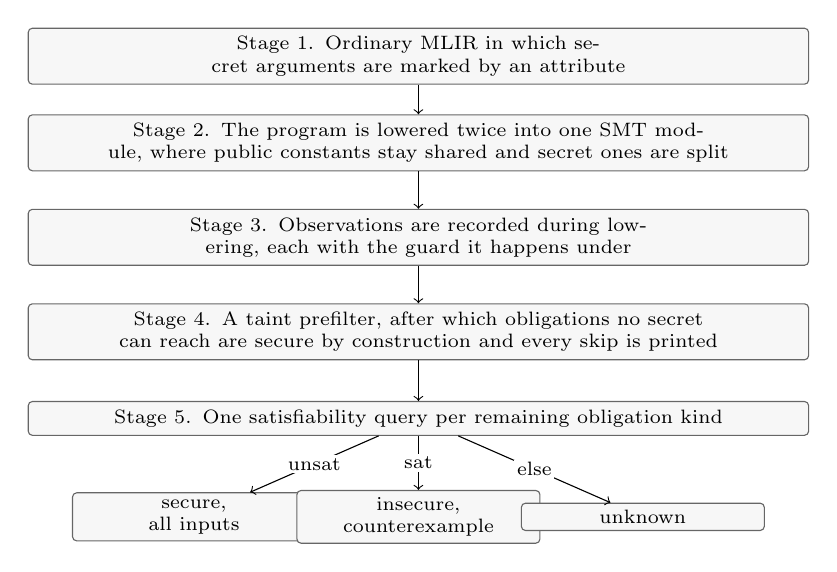
\begin{tikzpicture}[font=\scriptsize,line width=0.4pt,
  box/.style={draw=black!60,rounded corners=1.5pt,align=center,
              inner sep=3pt,text width=0.80\columnwidth,fill=black!3},
  vb/.style={draw=black!60,rounded corners=1.5pt,align=center,
             inner sep=2.5pt,text width=0.24\columnwidth,fill=black!3}]
  \node[box] (s1) at (0,0)
    {Stage 1. Ordinary MLIR in which secret arguments are marked by an
     attribute};
  \node[box] (s2) at (0,-1.10)
    {Stage 2. The program is lowered twice into one SMT module, where public
     constants stay shared and secret ones are split};
  \node[box] (s3) at (0,-2.30)
    {Stage 3. Observations are recorded during lowering, each with the guard it
     happens under};
  \node[box] (s4) at (0,-3.50)
    {Stage 4. A taint prefilter, after which obligations no secret can reach are
     secure by construction and every skip is printed};
  \node[box] (s5) at (0,-4.60)
    {Stage 5. One satisfiability query per remaining obligation kind};
  \node[vb] (v1) at (-2.85,-5.85) {secure,\\ all inputs};
  \node[vb] (v2) at (0,-5.85)     {insecure,\\ counterexample};
  \node[vb] (v3) at (2.85,-5.85)  {unknown};
  \draw[->] (s1) -- (s2);
  \draw[->] (s2) -- (s3);
  \draw[->] (s3) -- (s4);
  \draw[->] (s4) -- (s5);
  \draw[->] (s5) -- (v1) node[midway,fill=white,inner sep=1pt] {unsat};
  \draw[->] (s5) -- (v2) node[midway,fill=white,inner sep=1pt] {sat};
  \draw[->] (s5) -- (v3) node[midway,fill=white,inner sep=1pt] {else};
\end{tikzpicture}
\caption{The five stage protocol, in which the three answers a query can return are the three verdicts, so that nothing besides an unsatisfiable answer is ever folded into secure.}
\label{fig:protocol}
\end{figure}
The protocol consists of five stages, shown in Fig.~\ref{fig:protocol}.
Its input is an ordinary MLIR function with marked secrets, its output is one verdict per obligation kind, and the stages themselves separate what has to be trusted, the marking of secrets and the leakage model, from what is computed, the traces and the queries.
Since the obligations are never merged, a satisfiable answer arrives already sorted, and the counterexample itself names the observation, control, address, latency or resource, on which the two traces part ways, so that a separate diagnosis stage neither arises nor is needed.
\paragraph{Stage 1, mark the secrets}
The input is ordinary MLIR, in which a function argument carries an attribute declaring it secret while everything left unmarked counts as public, and the attribute is accepted in three spellings so that kernels arriving from neighbouring tools need no re annotation.
A kernel with no labels at all has no property that could be proved, so the tool answers unknown for it and never secure.
\paragraph{Stage 2, run the program twice, virtually}
Write leakage check $L(p,s)$ for the leakage trace of the kernel, that is, the sequence of observations recorded while it executes on public input $p$ and secret input $s$, where each entry consists of the operand named by the leakage model above together with the guard under which the operation was reached, and where the entries appear in execution order.
Leakage freedom is then a statement about a pair of executions that share their public part, \[ \forall\, \text{public } p,\ \text{secrets } s, s'. \quad L(p,s) = L(p,s'). \] To obtain both traces at once the kernel is lowered into the SMT module twice, so that every public argument becomes the same SMT constant in both runs, the initial memory remains one shared state, and every secret argument turns into two independent constants.
We share the public constants outright rather than declaring a pair of them and asserting their equality, because this keeps the formula small and the counterexamples readable, since the only free variables left are the ones the property allows to differ.
\paragraph{Stage 3, record observations during lowering}
Each operation is translated into its formula, and at exactly that moment the leakage model decides what the operation reveals, according to the four obligations set out above.
Observing therefore happens exactly where a formula is produced and nowhere else, which is why the same recorder works on symbolic rewrite patterns that never exist as concrete IR at all.
The guard attached to an observation is the conjunction of every branch condition on the path to it, and the same guard is what makes the value part of every rule conditional, so that an operation on an untaken path neither constrains its result nor disturbs the memory, and control flow can therefore be handled by if conversion without any path being executed twice over.
A bounded loop is unrolled to its bound, each iteration is guarded by the loop condition of all the iterations before it, and the number of iterations that survive those guards is itself recorded as a control observation, which is how a trip count that depends on a secret is caught by the same machinery as a secret branch.
\paragraph{Stage 4, the cheap check first, then one obligation at a time}
A taint prefilter walks the flattened program forward starting from the secret arguments, and wherever no secret can reach the observations of an obligation, neither through the observed value nor through the guard it happens under, that obligation is secure by construction, the solver call is skipped, and the skip itself is printed rather than silently absorbed.
The prefilter is meant to skip only answers that are already forced, and a test pins that disabling it leaves every verdict in our kernel suite unchanged, a property it did not have until it learned that a secret stored through an LLVM pointer and loaded back is still a secret.
Whatever the prefilter does not remove becomes one query per obligation kind, in which we take the observations of that kind from both traces, build the assertion that the traces agree, meaning that the guards coincide and that each guard implies equality of the observed value, then assert the negation of that and ask the solver for satisfiability.
Comparing the guards and not the values alone is what makes a pair of runs that took different paths surface immediately as a control violation, instead of showing up later as a spurious mismatch between values.
\paragraph{Stage 5, the verdict}
An unsatisfiable answer means secure, that is, proved for all inputs under the stated leakage model, a satisfiable answer means insecure and comes with the two secret values that separate the traces, which is a counterexample and not an alarm, and anything else is unknown and is never folded into secure.
Two reporting rules sit in the output for the same reason.
Every secure line prints how many observations of its kind existed at all, so that a vacuous verdict about a channel the kernel never touched cannot be mistaken for a channel that was checked, and a verdict whose loops were cut by the unroll bound is flagged as bounded.
Because the obligations are discharged separately, a verdict always names the channel it is about, and across the kernel corpus this separates a table lookup at a secret index, which yields an address verdict, from a secret branch, which yields a control verdict, from a secret divisor, which yields a latency verdict and is the KyberSlash mechanism named at the start of this section, whereas a single undifferentiated report would have said only that something leaks somewhere.
The index operands of every access are compared at bit granularity, which is strictly stronger than any real cache attacker, who resolves only lines of 64\,B~\cite{yarom2014flushreload}, although the choice between two memory references is not itself observed before lowering, so a secret that picks which buffer to read escapes the address obligation until the access becomes an LLVM pointer.
\subsection{Safe means both halves at once}
\label{sec:verify:property}
The leakage query compares observations and by its very construction cannot notice that a step changed the result, so a rewrite that returns a stale value adds no observation and passes the check.
The converse fails just as cleanly, since a rewrite that branches on a secret computes exactly the right answer and passes any equivalence check.
Each property on its own therefore certifies a genuine bug as safe, and for that reason we call a step specified only when both hold on its template, by two logically distinct queries that share the SMT encoding infrastructure.
The first query is semantic congruence, requiring that return values agree pairwise across the return sites actually taken and, unless a template declares itself about values only, as the memory to register templates must, that the memory left behind agrees as well, under a refinement criterion that tracks the polarity of undefined behaviour, in the manner of bounded translation validation for LLVM~\cite{lopes2021alive2}.
The second query is noninterference, that is, the self composition of \S\ref{sec:verify:protocol} already described.

A lowering step is not a rewrite of one fixed program but a structural specification over surrounding code, and we write it down as a source function and a target function whose unknown parts are left as holes, where a hole is an uninterpreted function tied across the two programs by congruence, and whose shapes, meaning extents, bounds, strides and widths, are swept over a declared set of values, so that a discharged obligation covers every instantiation of the holes at every swept shape.
Holes are pure functions of their arguments, so code that touches memory cannot hide inside one, and the sweep samples shapes rather than quantifying over them, since a symbolic stride is not representable in the dialects we check; a template is therefore a family of instances and not a proof about every program the pass will ever meet.
The encoding rests on four ingredients, namely guards attached to observations, congruence of holes, inclusion of returned values in the equivalence query, and the requirement that arguments be non poison and congruent exactly; removing the first or the third lets a leak or a wrong result pass, removing either of the other two produces false alarms, and each of the four is pinned by a mutation test that fails as soon as the ingredient is removed.
\subsection{Tools and scopes}
\label{sec:verify:tools}
The method is exposed through four tools, which ask the same question at four different scopes.
The kernel tool asks whether one given kernel is leak free and quantifies over all inputs of that one program.
The rewrite tool asks whether a rule preserves leak freedom and quantifies over every program the rule matches.
The lowering tool asks whether a step is safe on both halves and quantifies over every instantiation of its holes at every swept shape.
The coverage tool asks how much of a compiler is checkable at all and counts over a corpus of that compiler, which for the compilers below is their own test suite rather than a sample of real inputs.
The work reported here is done by the last two, and the first two serve mainly to supply them with tested ingredients.

The rewrite check needs no labelling of secrets whatsoever, because the bound is the leakage of the source program itself, in the form $L_S(x) = L_S(x') \Rightarrow L_T(x) = L_T(x')$, and it is this shape that lets a single proof cover every program the pattern matches.
Run on hand-written rewrite patterns, among them the reverse of a textbook strength reduction, that check finds rewrites which the upstream value verifier accepts and which nevertheless introduce a variable-latency division, since value correctness and constant time are different properties and only the first of them was being checked.

Coverage is the tool that puts a number on the cost of the method, sorting every operation occurrence in the corpus of a compiler into three forms.
Form 0 translates into SMT, which the tool establishes by actually lowering each occurrence in a probe function of its own types and attributes, form 1 is covered by a template proved once on both halves and reused afterwards, and form 2 is untranslatable today and marks the frontier where new work has to go.
Whether a semantics exists for an operation's name at all is a much weaker question, and we report that figure only as an upper bound, since a registered rule may still refuse the occurrence in front of it, as the memory rules do for dynamic shapes and for elements wider than a byte.
\subsection{Polygeist, end to end}
\label{sec:verify:polygeist}
We chose Polygeist as the pipeline to verify because, of the six MLIR based compilers we mapped, it had the largest share of operation mentions with a registered semantics by name, 61.9\,\% against 53.4\,\% for a homomorphic encryption compiler and 17.3\,\% for a PyTorch to MLIR front end.
The reason is structural rather than accidental, and it is that Polygeist speaks the shared MLIR dialects~\cite{lattner2021mlir} instead of a dialect of its own invention.
Measured by translation rather than by name the picture is far more sober: of the operation mentions in Polygeist's 89 lit test files, 74.4\,\% have a rule by name, but only 8.2\,\% translate, and 11 of its 51 test functions translate whole.
No step is yet checkable on the programs of that corpus, since the input of every step still contains an operation we cannot translate, with calls and floating point arithmetic as the largest blockers, and every result below is therefore about the templates and not about Polygeist's test programs.

Six of the eight steps carry a template together with a falsifying control, and the two that do not are blocked by the model rather than by effort, since both of them lower into parallel runtimes whereas the SMT memory model underneath every check here is sequential, so a specification written for them would be a fabrication.
We therefore report them as unknown with that reason attached, which is a different statement from saying that nobody has got round to them yet.

Every template is transcribed by hand from the source of the pass with a citation to file and line, is swept over between 4 and 36 shapes, and is paired with a control that violates its side condition.
Each control is refused by at least one half of the property, five of them by the equivalence half alone and one, the loop restructuring control, by the leakage half alone, although two headers had predicted otherwise, which is why the prediction is recorded before the run.
The transcription is the weak link, since a template that misstates the pass is checked just as readily as one that states it correctly, and nothing yet runs the pass itself on a template's source to confirm that it produces the template's target (\S\ref{sec:discussion}).
That discipline is what turns Table~\ref{tab:polygeist} into evidence instead of a summary, and it paid for itself, since four encoding faults were found not by inspection but by correct templates failing.
Congruence had been comparing poison bits instead of values, the source and the target of one run had been given different initial memories, stores under a guard had been executing on untaken paths, and accesses parked at index 0 on untaken paths had assumed that cell 0 of an argument is readable, and each fix left every verdict other than the one that exposed it unchanged.

The individual verdicts also show the two halves doing genuinely independent work.
The memory to register step removes an address channel, taking the source's 18 observations down to 4 in the first of its ten swept instances, and preserves values, while its stale forwarding control leaks no more than the original does, exactly as it must, and is therefore refuted by the equivalence half alone.
The loop restructuring step holds on both halves, and its do while control breaks the trace while leaving the values untouched, which is the mirror image, and it breaks it on the trip count, since a do while shape runs the body once before the condition is ever tested.
Loop canonicalization is the step whose side condition is about values, so when it is applied where that condition fails the body reads a stale value, and the leakage half correctly reports the step as preserving, since a wrong answer leaks no more than a right one, while only the equivalence half refutes it.

The final step lowers to LLVM, for whose integer operations SMT semantics already existed in the verification dialects, while its memory operations had none.
We supply the three this lowering emits, address computation, load and store, together with the pointer type, on the same memory model the memref side already uses, so that a memory reference and the pointer it lowers into are one and the same SMT value and one initial memory is shared across both sides.
The step is covered in slices, its arithmetic, its structured to unstructured control flow and its memory access, rather than end to end, and a kernel whose index is the secret comes back as breaking the address obligation once lowered, which shows the new leakage rule to be load bearing.
